\chapter{RecercaPrevia}
\label{c:RecercaPrevia}
\section{Què és la qualitat de l’aigua?}
La qualitat de l'aigua es un terme que es refereix a les caracteristicas fisicas, quimicas y bilogicas de l'aigua. Per determinar-la, s'analitzan alguns paràmetres.

Segons Wikipedia \cite{WikiAgua}, s'entén la qualitat de l'aigua com `característiques químiques, físiques, biològiques i radiològiques de l'aigua`, en relació amb necessitats humanes.

La Fundació Aquae \cite{Fundacionaquae} indica que es tracta d'un conjunt de paràmetres, com temperatura, contingut mineral i bacteris, mesurats i comparats amb estàndards, per definir si l'aigua és apta per a fins determinats o no.

En aquest TR analitzarem diversos paràmetres per analitzar la qualitat de l'aigua que es classifiquen en tres grups:
\begin{enumerate}
  \item \textbf{Paràmetres químics}: són els relacionats amb la composició química de l’aigua; indiquen si és potable o contaminada. En concret, estudiarem el pH, la duresa, els nitrats i els nitrits, el clor i els metalls pesants. Els paràmetres químics seran explicats a la secció~\ref{sec:pq}.
  \item \textbf{Paràmetres físics}: mesuren característiques visibles o mesurables sense canviar la composició de l’aigua. Els paràmetres físics seran explicats a la secció~\ref{sec:pf}. En aquesta secció, estudiarem la importància de la temperatura, el color, l’olor i el sabor en la qualitat de l’aigua.
  \item \textbf{Paràmetres biològics}: indiquen la presència de microorganismes que poden ser patògens. Els paràmetres biològics seran explicats a la secció~\ref{sec:pb}. En aquesta secció, explorarem els coliformes fecals, els protozous presents en l’aigua i els bioindicadors.
\end{enumerate}


\section{Paràmetres químics} \label{sec:pq}

\subsection{Què és el pH i per què és important?}
El pH és una mesura que serveix per establir el nivell d’acidesa o alcalinitat d'una dissolució. La `p` ve de `potencial` i l'`H` ve de l’àtom d’hidrogen, per això el pH és el potencial de l’hidrogen.

S'expressa com el logaritme negatiu de base 10 de la concentració de ions d'hidrogen: $ \text{pH} = -\log_{10} [\mathrm{H}^+] $.

A la fórmula la ${H}^+$ és la concentració de ions d'hidrogen en la solució, mesurat en mols per litre (mol/L). $-\log_{10}$ és el logaritme en base 10, el signe negatiu s'utilitza amb l'objectiu que el pH sigui un número positiu. La raó és perquè el logaritme d'un número menor que 1 és negatiu.

D'altra part, el \textbf{pOH} és una mesura de concentració de ions hidroxil ${OH}^-$ en una dissolució. S'expressa com el logaritme negatiu de base 10 de la concentració de ions hidroxil, i a diferència del pH, s'utilitza per mesurar el nivell d’alcalinitat d'una dissolució. Es calcula amb la formula  $ \text{pOH} = -\log_{10} [\mathrm{OH}^-] $.
\subsubsection{ Quina relació hi ha entre el nivell d'acidesa i el pH?}
Les dissolucions àcides tenen una alta quantitat de ions d'hidrogen. Això significa que tenen baixos valors de pH, i per tant, el seu nivell d'acidesa és elevat. Així que una dissolució serà més o menys àcida depenent de la quantitat d'hidrogen que contingui aquesta.

D'altra banda, les dissolucions bàsiques (alcalines) tenen baixes quantitats de ions d'hidrogen. Això vol dir que tenen alts valors de pH, i per tant el seu nivell d'acidesa és baix.
\subsubsection{Escala del pH}
\begin{figure}[h!]
\centering
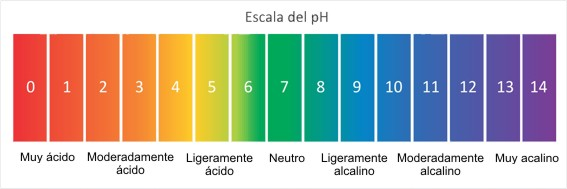
\includegraphics[width=0.9\textwidth]{./Figures/EscaladepH.png}
\caption{Escala del pH}
\label{fig:escaladeph}
\end{figure}
L'escala de pH s'utilitza per mesurar el grau d'acidesa d'una dissolució, i com que el pH està relacionat amb el pOH, coneixent el grau d'acidesa d'una dissolució, també podem saber el seu grau d'alcalinitat (basicitat).

Com podem observar a la figura \ref{fig:escaladeph}, el valor del pH va del 0 al 14. Les substàncies amb pH igual a 0 són més àcides; les que tenen el pH = 7 són neutres, i les que tenen pH = 14 són les menys àcides, per tant, són les més bàsiques.

\subsubsection{Què ens diu el pH sobre la qualitat de l'aigua?}
El pH és un paràmetre fonamental entre els paràmetres; com he dit abans, indica el grau d'acidesa o alcalinitat. El pH depèn de la quantitat d'hidrogen que conté l'aigua.

Un pH d'1 ens diu que la substància és molt àcida i, per tant, perillosa. L'àcid clorhídric (HCl(aq)) té aproximadament aquest pH. A l'altre extrem de l'escala, amb un pH aproximat de 14, tenim sosa càustica (NaOH). Gràcies a l'escala de pH (figura \ref{fig:escaladeph}), podem saber si la dissolució és més àcida o bàsica. En general, un pH de 7, és a dir, neutre, seria el més òptim en la majoria dels casos; és un pH similar al del nostre cos, la suor, etc.
\subsubsection{Instrument de mesura}
El \textbf{pH-metre} és un instrument utilitzat per mesurar el pH d’una dissolució. Va ser construït per \textbf{Arnold Orville Beckman} l’any \textit{1934}.
\begin{figure}[H]
\centering
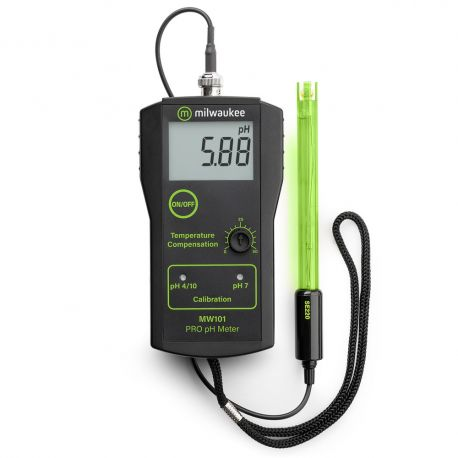
\includegraphics[width=0.3\textwidth]{./Figures/pHmetre.png}
\caption{Imatge del pH-metre actual}
\label{fig:pH-metre}
\end{figure}
El model de Beckman era més gran que el model actual del pH-metre
\begin{figure}[H]
\centering
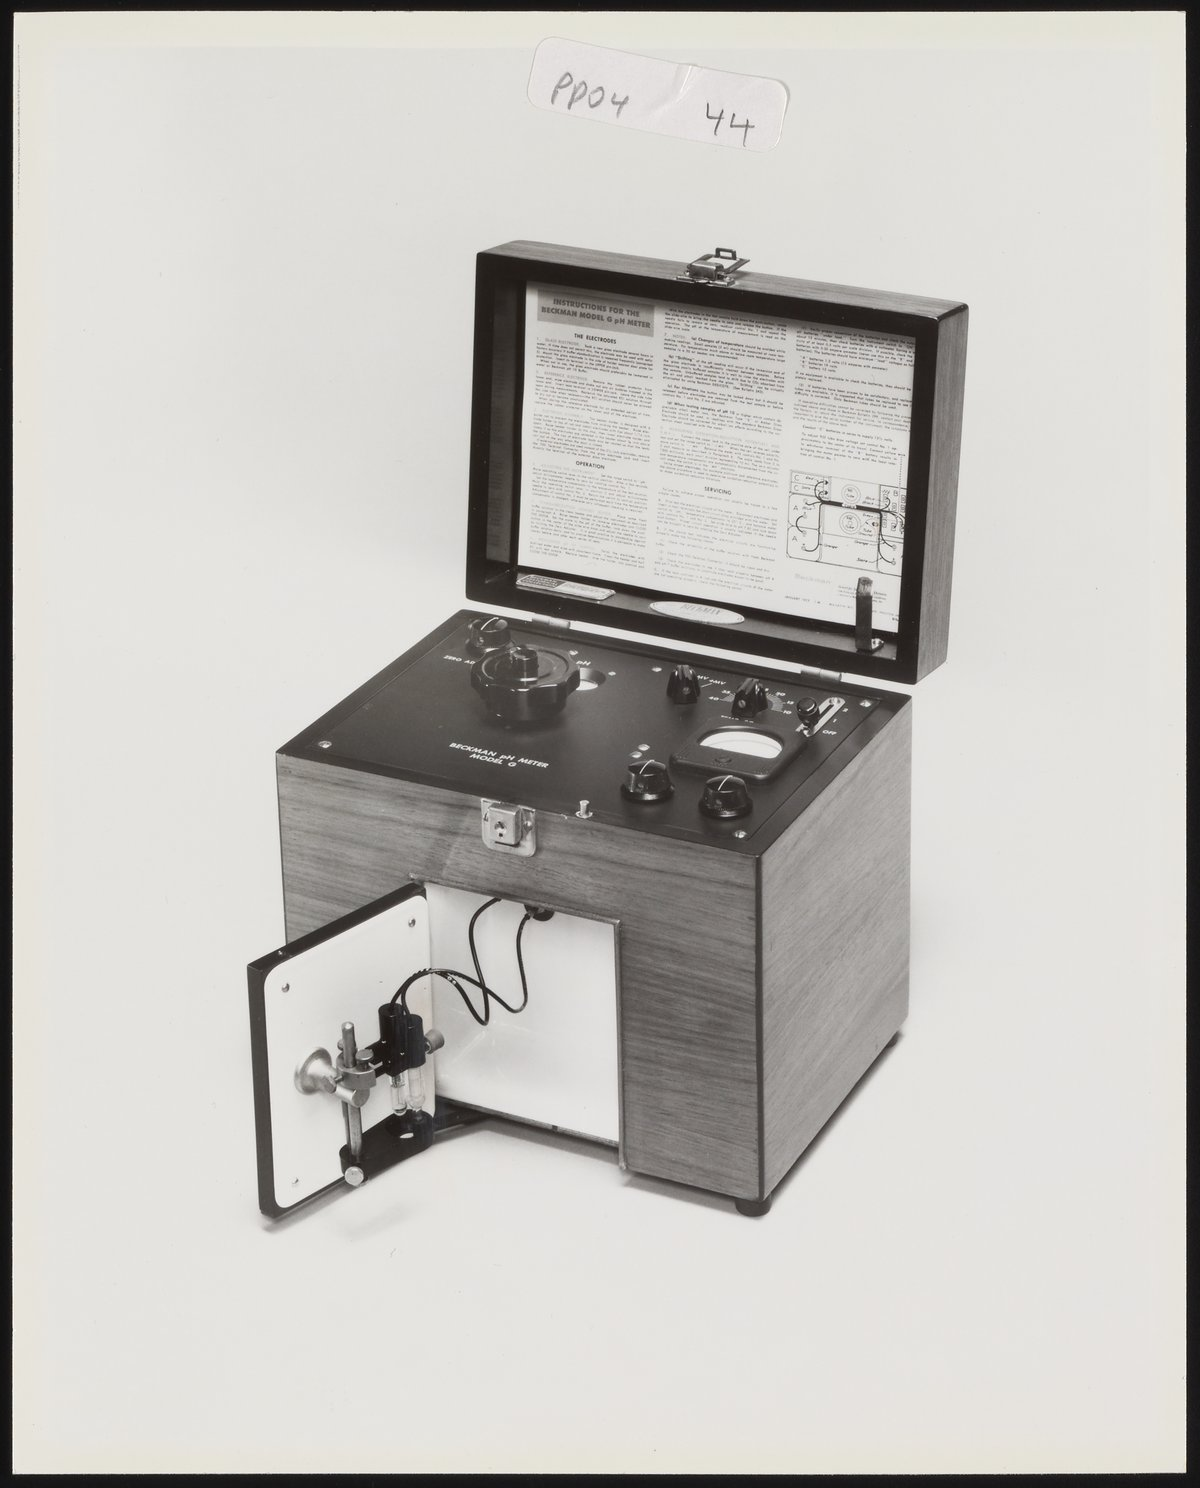
\includegraphics[width=0.3\textwidth]{./Figures/modelbeckman.png}
\caption{Imatge del pH-metre (model de Beckamn)}
\label{fig:pH-metre}
\end{figure}

\subsection{Què és la duresa de l’aigua i com ens afecta?} \label{subsec:duresa}
Es la concentració de compostos minerals en una certa quantitat d'aigua, especialments sals de magnesi i calci.\\
\textit{Fonts:} \cite{Fasca}\\
L'aigua `dura` te una alta concentracio d'aquestes sals i l'aigua `suau`, te una concentracio baixa d'aquestes. La duresa es pot calcular amb la seguennt formula: (mg/L de Calci (Ca) + mg/L de Magensi (Mg) x 4.2 )/10
\subsubsection{Què ens diu la OMS?}
L'Organització Mundial de la Salut no considera que la duresa de l'aigua tingui un impacte negatiu en l'organisme . En una guia, afirma que els paràmetres per al consum oscil·len entre 100 i 300 mg/l de carbonat de calci, encara que el llindar de tolerància pot estar per sobre o per sota en funció de la normativa de cada país.

En general, la concentració desitjable es considera inferior a 100 mg/l (aigua de més qualitat) i que per sobre de 500 mg/l qualitat ja no és acceptable. En el cas concret d'Espanya, la normativa tecnicològica-sanitària estableix un valor de contingut de calci de fins a 100 mg/l amb un límit màxim de tolerància de 200 mg/l. \\
\textit{Fonts:} \cite{Fasca}
\subsubsection{Instrument de mesura}
Per mesurar la duresa podem utilitzar els \textbf{test kits de duresa}.
Es un conjunt d’eines i reactius que s’utilitzen per determinar la quantitat de calci i magnesi.
Amb aquestes dades y utlitzand la formula; (mg/L de Calci (Ca) + mg/L de Magensi (Mg) x 4.2 )/10, poden determinar el nivell de duresa de una dissolució.
\begin{figure}[H]
\centering
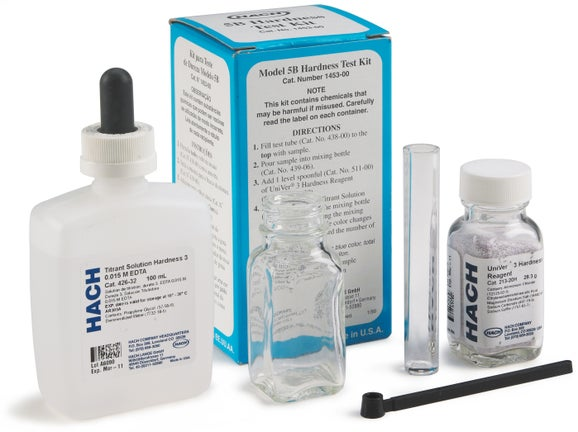
\includegraphics[width=0.3\textwidth]{./Figures/testduresa.png}
\caption{Imatge del kit de duresa}
\label{fig:kitsduresa}
\end{figure}

\subsection{Què són els nitrats i nitrits i per què ens han de preocupar?} \label{subsec:nitratsnitrits}
El nitrat \(\mathrm{NO_3^-}\) és un compost químic format bàsicament per nitrogen i oxigen. Naturalment es troba en el sòl i l'aigua, per la qual cosa és un nutrient fonamental per a molts éssers vius.

Quan paguem la terra per millorar el seu rendiment, utilitzem productes de nitrogen, ja siguin fertilitzants minerals o orgànics com els fems. A aquest augment de nitrats, hem d'afegir el plus que representa nitrogen contingut en aigua de reg (aigua utilitzada per el reg de conreus o jardins). Per tant, el nivell final d'aquest compost pot ser alt en moltes ocasions.

Amb el temps, i essencialment a causa de l'acció d'alguns bacteris, aquests nitrats evolucionen en nitrits \(\mathrm{NO_2^-}\), ions considerats més tòxics.
\subsubsection{El nitrit i les seves conseqüències}
El nitrit s'origina en les fruites profundes que es produeixen quan el sistema de reg mou el nitrat al sòl. Aquest risc és més alt quan s'utilitza el reg de la superfície. La contaminació de l'aigua superficial pot tenir conseqüències tan greus com la mort de la fauna aquàtica a llarg termini.

Com hem vist, l'excés de nitrit pot causar la seva contaminació a l'aigua, però també als cultius que estan regats amb aquesta aigua contaminada. Per tant, moltes verdures es poden veure afectades.

Aquestes grans quantitats de nitrits a l'aigua poden tenir un impacte negatiu en la salut de les persones. Per evitar problemes, l'OMS recomana un límit de 50 mil·ligrams de nitrat per litre.\\
\textit{Fonts:} \cite{Scielo}: en aquest treball es menciona la recomanació de l'OMS sobre el nitrat.
\subsubsection{Instrument de mesura}
Per mesurar el nitrat i el nitrit podem utilitzar un \textbf{kit de prova de nitrat-nitrit}, que són mètodes per mesurar aquests elements amb més precisió.
\begin{figure}[H]
\centering
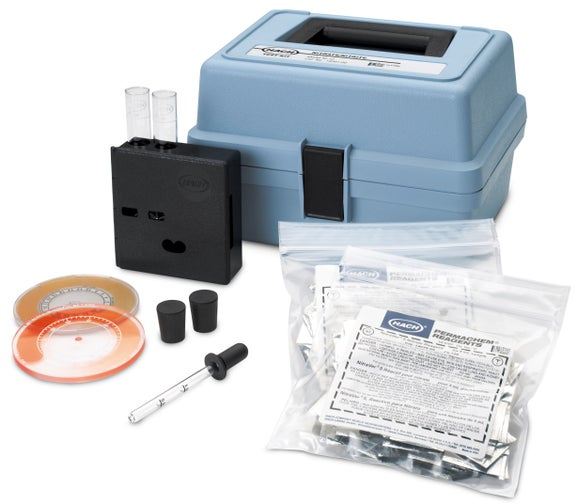
\includegraphics[width=0.3\textwidth]{./Figures/nitratnitrit.png}
\caption{Imatge de kit de prova de nitrat-nitrit}
\label{fig:kitnitrats}
\end{figure}

\subsection{Clor: per què és essencial en l’aigua que bevem?} \label{subsec:clor}
El clor és un element químic, un gas groc verdós, dens i amb una olor irritant. S'utilitza principalment per desinfectar l'aigua, eliminant així les bacteris i altres microorganismes nocius.

La seva presència és considerada l'últim pas per a la potabilització de l'aigua. Desinfecta microorganismes patògens que causen malalties als humans; per aquesta raó, la seva desinfecció és fonamental en la protecció de la salut pública.

Tot i que existeixen altres mètodes de desinfecció, el clor ha sigut el responsable de l'augment de l'esperança de vida a l'Europa del passat segle XX. Però, anteriorment, fa cinc segles, s'utilitzaven altres formes de desinfecció més rudimentàries, com bullir l'aigua.

La revista Rain of life \cite{RoF} classifica el logre de la cloració (procés de desinfecció que utilitza clor) com “probablement el més significatiu progrés de la salut pública del mil·lenni” l'any 1997.

Per tant, el clor és un producte químic amb l'objectiu de desinfectar l'aigua. Tanmateix, l'ús d'aquest component químic \textbf{no és segur.}
\subsubsection{Com el clor de l'aigua potable afecta la salut}
Segons el doctor en Medicina Josep Lluís Berdonces, qui es basa en diferents estudis sobre aquest tema, la cloració de l’aigua pot tenir efectes nocius sobre la salut de les persones. Té en la seva composició àcids húmics i fúlvics. Les conseqüències d’aquests components químics sobre la salut humana són variades. Molts d’ells tenen una gran afinitat per unir-se amb els diversos greixos del cos.\\
\textit{Fonts:} \cite{RoF}
\subsubsection{Instrument de mesura}
Per mesurar el clor, podem utilitzar un \textbf{fotòmetre portàtil de clor}.
\begin{figure}[H]
\centering
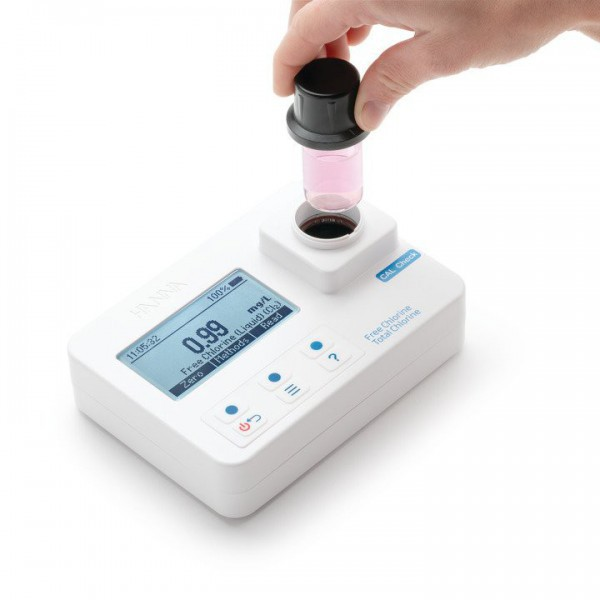
\includegraphics[width=0.3\textwidth]{./Figures/Cloro.jpg}
\caption{Imatge del fotòmetre portàtil de clor}
\label{fig:clormetre}
\end{figure}

\subsection{Presència i efectes dels metalls pesants en l’aigua potable} \label{subsec:metallspesats}
El terme de `metalls pesants` es refereix a qualsevol element químic metàl·lic que té una alta densitat i pot ser tòxic o verinós a baixes concentracions.

Alguns metalls pesants com el coure ($Cu$), el seleni ($Se$), i el zinc ($Zn$) són essencials per mantenir el metabolisme del cos humà. No obstant això, en altes quantitats poden conduir a l'enverinament. Aquesta intoxicació pot ocórrer si es consumeix aigua amb algun d’aquests metalls.
\subsubsection{Com es contamina l’aigua amb metalls pesants?}
El principal motiu és la contaminació industrial. Una altra font de contaminació pot ser els abocaments d'aigües residuals. Hi ha casos en què l’aigua pateix un procés d’enriquiment de metalls pesants, ja que passa per roques que contenen aquests metalls en la seva composició.
\subsubsection{Alguns metalls pesants presents a l'aigua}
\begin{enumerate}
 \item \textit{\textbf{Alumini}}
 Tot i que l'alumini no és un metall pesat, representa aproximadament el 8 per cent de la superfície terrestre i és el tercer element més abundant. Està disponible per a la ingestió humana a través de l'aigua potable.
 \item \textit{\textbf{Arsènic}}
 L'arsènic és la causa més freqüent d'enverinament per metalls pesants aguts en adults. L'arsènic també es pot trobar en el subministrament d'aigua, el que porta a l'exposició en marisc, bacallà, haddock i alguns altres aliments marins
 \item \textit{\textbf{Coure}}
 El coure a altes concentracions pot ser tòxic. Els efectes per a la salut són els següents: pot causar vòmits, diarrea, pèrdua de força o, per a l'exposició severa, la cirrosi del fetge.
 \item \textit{\textbf{Ferro}}
 El ferro és un metall pesant comú a l'aigua, s'ha de tenir cura de menjar suplements de ferro, i en la dieta pot enverinar agudament els nens petits. La ingestió representa la major intoxicació per ferro per a les persones.
 \item \textit{\textbf{Mercuri}}
 El mercuri es genera naturalment en el medi ambient en la desgasificació de l'escorça terrestre i les emissions volcàniques.
\end{enumerate}
\textit{Fonts:~\cite{WikiMetales},~\cite{carbotecnia}}
\subsubsection{Instrument de mesura}
Per mesurar els metalls pesants (no tots) podem utilitzar un \textbf{kit d’anàlisi de metalls pesants}, que encara que aquests kits no proporcionin un valor exacte, podem aproximar-lo i així mesurar els nostres metalls pesants.
\begin{figure}[H]
\centering
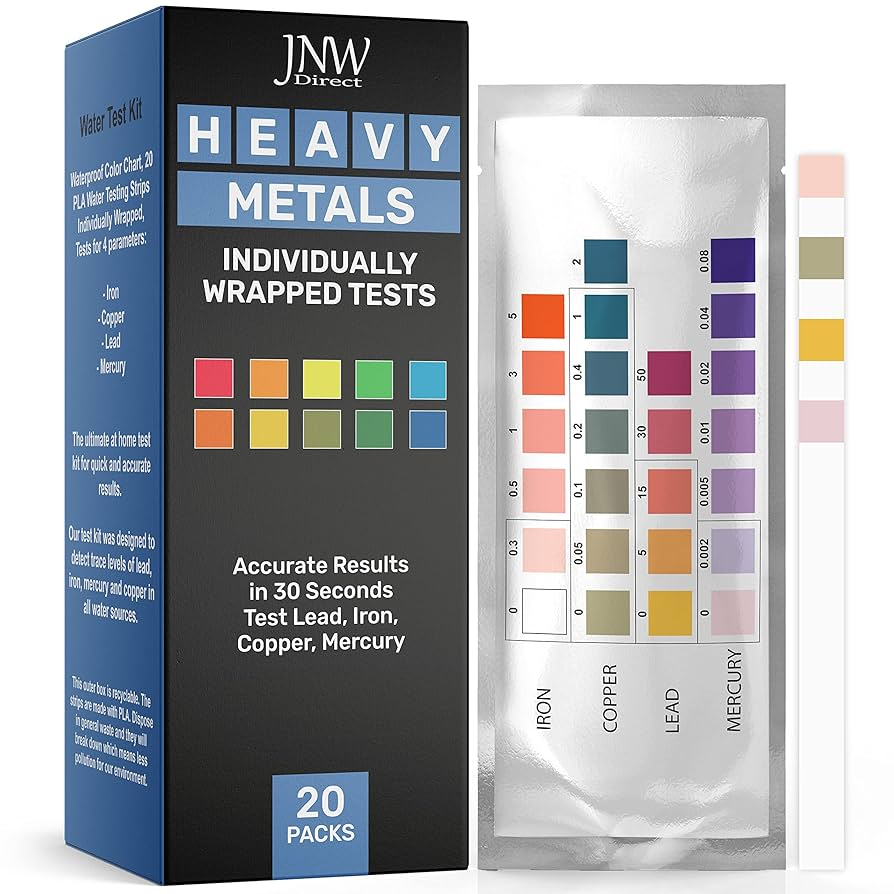
\includegraphics[width=0.3\textwidth]{./Figures/metales.jpg}
\caption{Imatge de kit d’anàlisi de metalls pesants}
\label{fig:kitmetall}
\end{figure}
\section{Paràmetres físics} \label{sec:pf}

\subsection{Temperatura de l’aigua: què ens diu sobre la vida aquàtica?} \label{subsec:temperatura}
La temperatura és un paràmetre físic que permet mesurar les sensacions de calor o fred. En termes científics, és una mesura de l’energia cinètica de les molècules que el componen, és a dir, com de molt es mouen o s’agiten aquestes molècules.
\subsubsection{Quina relació te amb la qualitat de l'aigua?}
Un gran exemple de la importància de la temperatura és a la vida aquàtica. Per exemple, l’aigua freda reté més oxigen; això fa que sigui vital per als peixos i altres éssers aquàtics. Quan aquesta temperatura augmenta, la quantitat d’oxigen disminueix, afectant així la supervivència d’aquests organismes.

També afecta el metabolisme dels organismes: els animals aquàtics i les plantes tenen un rang de temperatura ideal. Si aquest rang és superat per molt de temps, els organismes poden patir malalties o fins i tot aquest canvi pot portar-los a la mort.

Una dada curiosa és que, a temperatures més altes, algunes substàncies tòxiques es tornen més actives o més perilloses per als organismes.\\
\textit{Fonts:} \cite{UCM}

\subsection{Color de l’aigua: què ens indica sobre la seva qualitat?} \label{subsec:color}
És un dels paràmetres \textbf{organolèptics} (organolèptics són les característiques d'un producte que es pot percebre amb els sentits, en aquest cas, la vista) que indica la qualitat de l'aigua per al consum humà. Està relacionat amb les substàncies dissoltes o les \textbf{partícules en suspensió} (són partícules sòlides o líquides molt petites disperses en l’aire).
\subsubsection{La seva importància amb la qualitat de l'aigua}
El color és important perquè pot alertar sobre la presència de substàncies que, en combinar-se amb desinfectants com el clor (més informació sobre el clor al apartat~\ref{subsec:clor}), poden generar \textbf{subproductes nocius}.

`Els compostos com ferro, manganès o coure, i especialment les substàncies húmiques (àcids fúlvics i húmics), són els principals responsables del color. Tot i que aquestes substàncies són inofensives per si soles, poden formar compostos tòxics durant la desinfecció amb clor.` (Higiene Ambiental, 2019, \textit{Color del agua, parámetro indicador de calidad}\\
 \textit{Fonts:} \cite{HA}

\subsection{Què ens diu l’olor i el sabor de l’aigua?} \label{subsec:olorisabor}
L’olor i el sabor són, com el color, \textbf{paràmetres organolèptics} essencials en l’avaluació de la qualitat de l’aigua. La presència d’olors i sabors inusuals pot indicar possibles problemes de contaminació o alteració biològica, i s’hauria de considerar una alerta sanitària, fins i tot si l’aigua compleix amb els altres paràmetres químics i biològics.

\section{Paràmetres biològics} \label{sec:pb}
\subsection{Coliformes fecals: què ens diuen sobre l’aigua que bevem?} \label{subsec:coliformes}
Els coliformes fecals són bacteris coliformes que estan presents a l’intestí dels animals de sang calenta (humans, gossos, vaques, ànecs, etc.). Aquests bacteris surten del cos a través dels excrements.

La raó per la qual són tan importants en l’aigua és perquè, si es detecten coliformes fecals, això indica que hi ha una contaminació amb matèria fecal i, per tant, hi ha un major risc de presència d’altres microorganismes perillosos, com virus o paràsits.
\subsubsection{Malalties que poden causar els bacteris coliformes}
\begin{enumerate}
 \item \textit{\textbf{Gastrointestals}} que causen diarrea i vòmits.
 \item \textit{\textbf{La disenteria}}, és una afecció inflamatòria de l’intestí, especialment del còlon, que produeix diarrea greu amb moc o sang als excrements.
 \item \textit{\textbf{Virus}}, que poden causar hepatitis.
\end{enumerate}
\textbf{En conclusió}, la presència de bacteris coliformes pot indicar la presència d'altres patògens més perillosos, com E. coli (és un tipus de bacteri que pot produir malalties i causar diarrea).
\subsection{Protozous a l’aigua} \label{subsec:protozous}
A l’aigua es poden trobar microorganismes com els protozous, alguns d’aquests poden ser patògens i poden causar malalties gastrointestinals si s’ingereixen. Alguns exemples d’aquests protozous són el Giardia, Cryptosporidium, Entamoeba histolytica i Toxoplasma gondii. Però la majoria dels protozous no representen un risc per a la salut humana, i es troben comunament en ambients aquàtics.
\subsection{Bioindicadors} \label{subsec:indicadorbiologic}
Un indicador biològic o \textbf{bioindicador} de l’aigua són organismes vius que poden utilitzar-se per avaluar la qualitat de l’aigua. Aquests organismes poden proporcionar informació sobre la presència de contaminants o l’estat general de l’ecosistema aquàtic.

Una vegada explicat què vol dir qualitat de l’aigua i alguns dels paràmetres més importants, donaré una mica més de context i la importància global de la qualitat de l’aigua.

\section{OMS (Organització Mundial de la Salut)}
És un organisme especialitzat de les Nacions Unides que es dedica a la salut a nivell mundial. El seu objectiu principal és que totes les persones assoleixin el màxim grau de salut possible.
\subsection{Estàndards de la qualitat de l’aigua de l’OMS}
Des de 1958, la OMS (Organització Mundial de la Salut) va establir uns estàndards per a la qualitat de l’\textbf{aigua potable} que serveixen com a referència \textbf{internacional} per garantir la seguretat i potabilitat de l’aigua.
\subsubsection{Què són realment els estàndards per a l’aigua potable?}
Són regulacions establertes per la legislació interna dels països per controlar el nivell de contaminants a l’aigua de consum humà en cada nació.

Els estàndards nacionals se centren en l’establiment de límits per regular els contaminants que presenten un gran risc d’afectar la salut pública, i aquests es basen en la seva factibilitat segons els recursos econòmics i ambientals disponibles per a cada país.

Per establir aquests estàndards, la OMS va haver de realitzar una investigació i una anàlisi que els permetessin verificar si aquests estàndards complirien la seva missió principal: protegir la salut pública. La OMS s’encarrega únicament de concentrar i establir les pautes, les quals són adaptables pels països. Els països poden escollir lliurement si establir aquestes normes o no, ja que el país també té dret d’establir les seves pròpies normes, les quals poden ser menors, iguals i/o més estrictes que les recomanades per la OMS.
\subsubsection{Estàndards establerts per l’OMS}
\textbf{Coliformes fecals:} La quantitat de coliformes fecals recomanada per les guies de l’OMS és de 0 UFC (unitats formadores de colònies) / 100 ml.\\

\textbf{Arsènic:} L’estàndard establert per l’OMS per a l’arsènic a l’aigua és de 0,01 mg/L.\\

\textbf{Cadmi}: És un dels metalls més tòxics i és biopersistent. El nivell establert per l’OMS és de 0,003 mg/L, el qual és adoptat pel 38,88 per cent dels països. \\

\textbf{Cianur:} És una substància química potencialment letal que actua com a tòxic mitjançant la inhibició de certes proteïnes. Les quantitats de cianur permeses als països presenten una alta variabilitat. El valor recomanat per l'OMS es de 0,07 mg/L.\\

\textbf{Coure:}  El coure és un metall important perquè posseeix propietats que el fan extraordinàriament útil per a una diversitat d’usos. El nivell recomanat de coure per l’OMS és de 2 mg/L, el qual és adoptat pel 26,31 per cent dels països.\\

\textbf{Crom:} És un metall que es troba espontàniament a l’aigua, al sòl i a les roques. Les guies de l’OMS estableixen un nivell màxim recomanable de 0,05 mg/L.\\

\textbf{Mercuri:} Metall que ocorre de forma natural en l’ambient i que té diverses formes químiques. El nivell establert per l’OMS és de 0,001 mg/L.\\

\textbf{Nitrat:} Entre un rang de 10 mg/L i un màxim de 50 mg/L. Això permet inferir que el nivell de nitrats està ben administrat per les legislacions nacionals de cadascun dels països, els quals es mantenen dins dels estàndards de l’OMS.\\

\textbf{Nitrit:} L’estàndard establert per l’OMS és de 3 mg/L.\\

\textbf{Plom:} És un metall tòxic i molt perillós per a la salut. El plom entra a l’aigua potable primordialment com a resultat de la corrosió o desgast dels materials que estan al sistema de subministrament d’aigua. La concentració de plom recomanada per l’OMS és de 0,01 mg/L.\\

\textbf{Seleni:} És un micromineral antioxidant que prevé les reaccions excessives d’oxidació. L’OMS va establir un nivell de 0,01 mg/L.\\

\textbf{Alumini:} La recomanació de l’OMS és permetre com a màxim 0,2 mg/L perquè no cause cap dany a la salut humana.\\

\textbf{Amoniac:} És un gas incolor reconegut per molta gent, ja que s’utilitza en sals aromàtiques. L’OMS estableix una concentració màxima de 1,5 mg/L.\\

\textbf{Clorur:} El clorur és una sal composta per dos elements, un dels quals és el clor. Totes les sals de clorur són molt solubles en aigua. La concentració màxima recomanada per l’OMS és de 250 mg/L.\\

\textbf{Ferro:} És un dels minerals més abundants de l’escorça terrestre. És molt freqüent en les aigües subterrànies. L’OMS recomana 0,3 mg/L.\\

\textbf{Sodi:} És un metall tou, reactiu i de punt de fusió baix. Com que el sodi és explosiu i tòxic a l’aigua, l’OMS recomana un nivell màxim de concentració de 200 mg/L.\\

\textbf{Zinc:} L’OMS recomana una concentració màxima de 3 mg/L.\\

\textbf{Color:} Les guies de l’OMS recomanen un límit màxim de 15 UCV (unitats de color veritable).\\

\textit{\textbf{FONTS:}} \cite{Estan}

\subsection{Impacte global en la salut publica}
Es important mencionar l'impacte en la salut publica, com la mala qualitat de l'aigua afecta la salut globalment.
\subsubsection{Informació general}
L'aigua segura i fàcilment accessible és important per a la salut pública, ja sigui utilitzada per beure, per a ús domèstic, per produir aliments o amb finalitats recreatives. La millora de l'oferta, el \textbf{sanejament} (el sanejament és l’eliminació segura d’aigües residuals i deixalles.) i la gestió dels recursos hídrics poden impulsar el creixement econòmic dels països i contribuir en gran mesura a la reducció de la pobresa. \\
\textit{Fonts:} \cite{OrgaMS}

El 2010, l'Assemblea General de les Nacions Unides va reconèixer explícitament el dret humà al subministrament d'aigua i al sanejament. Totes les persones tenen dret a una disponibilitat contínua de quantitats suficients d'aigua segura, físicament accessible, assequible i d'una qualitat acceptable per a ús personal i domèstic.\\
\textit{Fonts:} \cite{OrgaMS}

\subsubsection{Aigua y salut}
L’aigua contaminada contribueix a la transmissió de malalties com les anteriorment mencionades. Si no es gestiona de forma apropiada, la població queda exposada a riscos per a la salut que, en realitat, es poden prevenir.

La mala gestió de les aigües residuals provoca que milions de persones consumeixin aigua amb contaminació biològica i química, incloent-hi arsènic, fluorurs i plom.

Segons l’OMS, cada any al voltant d’un milió de persones moren a causa de malalties diarreiques relacionades amb l’aigua insalubre, el sanejament deficient o la mala higiene de mans, provocant així unes 395 000 morts de nens menors de cinc anys. Hi ha malalties, com l’esquistosomiasi, que es transmeten pel contacte amb aigua infestada.
En definitiva, garantir l’accés a aigua potable segura no només és una necessitat bàsica, sinó també una de les mesures de salut pública més eficaces per prevenir malalties i salvar vides.

\subsection{Accions de l’OMS per Garantir Aigua Segura i Salut Pública}
L’OMS treballa arreu del món per evitar malalties causades per l’aigua contaminada i ajudar els governs a fixar normes i objectius que protegeixin la salut. Publica recomanacions sobre la qualitat de l’aigua per beure, reutilitzar aigües residuals de forma segura i per activitats recreatives, amb un enfocament basat en prevenir riscos.

Des del 2004, les seves \textit{Guies de qualitat de l’aigua de consum humà} expliquen com establir objectius de salut, fer plans per garantir que l’aigua sigui segura des que es capta fins que arriba a la llar, i fer controls independents per comprovar que tot funciona bé. L’OMS dona suport als països amb materials pràctics, ajuda directa, lleis adaptades a cada lloc i reforç de la vigilància.

Des del 2014, revisa productes per tractar aigua a casa, assegurant que eliminin microbis perillosos i ajudant els països a usar-los correctament.

També treballa amb \textbf{UNICEF} (Fons de les Nacions Unides per a la Infància (\textit{United Nations International Children's Emergency Fund})) per millorar l’aigua, el sanejament i la higiene als centres de salut. El 2015 van crear l’eina \textbf{WASH FIT} perquè centres petits, sobretot en països amb pocs recursos, puguin revisar els seus serveis, detectar problemes i aplicar millores concretes. Un informe del 2023 dona idees pràctiques per aconseguir aigua segura, sanejament i higiene en aquests centres.

\subsection{WASH FIT}
És una guia pràctica de l’Organització Mundial de la Salut (OMS) i UNICEF per millorar la qualitat de l’atenció sanitària en establiments de salut de països amb ingressos baixos i mitjans. Es centra en l’aigua, el sanejament, la higiene i la gestió de residus, utilitzant un enfocament de gestió de riscos per identificar, avaluar i abordar problemes relacionats amb aquests aspectes.

\subsubsection{Paîsos on s'ha utilitzat aquesta guia}
WASH FIT s’ha utilitzat en més de 40 països de tots els continents. Països com: \\
Benín, Bhutan, Burundi, Burkina Faso, Cambodja, Txad, Comores, República Democràtica del Congo, Equador, Etiòpia, Filipines, Ghana, Guatemala, Guinea, Guinea Bissau, Haití, Índia, Indonèsia, l’Iraq, Kenya, Libèria, Madagascar, Malawi, Maldives, Mali, Mauritània, Moçambic, Myanmar, Nepal, Nicaragua, Níger, Perú, República Democràtica Popular Lao, Ruanda, Sierra Leone, Sudan del Sud, Tanzània, Tadjikistan, Togo, Uganda, Veneçuela, Vietnam, Zàmbia i Zimbabwe. \\

Aquí dono per finalitzada la meva part de RecercaPrevia, la veritat és que he après molts conceptes i moltes coses que no sabia sobre la qualitat de l’aigua i alguns elements químics i biològics. A continuació, començaré la meva part pràctica, uns \textbf{3 experiments} que duré a casa per intentar, com bé he dit abans, mesurar la qualitat de l’aigua.
